\documentclass[12pt]{amsart}

\usepackage{a4wide, amsxtra}

\usepackage[pdftex]{graphicx}

\usepackage{hyperref}

 \title{MATH101 Assignment 10}

 \author{Mark Villar}

\begin{document} 

\maketitle 

\begin{enumerate}
	
	\item 
	
		\begin{enumerate}
		
			\item $\vec{PQ}=[1-(-1), 0-0, 0-0] = [2, 0, 0] = 2\mathbf{i}$ \\
			
				$\vec{PR}=[1-(-1), 1-0,1-0] = [2, 1, 1] = 2\mathbf{i}+\mathbf{j}+\mathbf{k}$ \\
			\item Let $\mathbf{u}=\vec{PQ}$ and $\mathbf{v}=\vec{PR}$. Then the orthogonal projection of 				$\mathbf{u}$ onto $\mathbf{v}$ is \\
				\begin{align}
					\mathbf{u^*}=\text{proj}_{\mathbf{v}} \mathbf{u}&=
					\frac{\mathbf{u}\cdot\mathbf{v}}{\|\mathbf{v}\|^2}\hspace{0.1cm} \mathbf{v}=
					\frac{4+0+0}{\left(\sqrt{4+1+1}\right)^2}\hspace{0.1cm}\mathbf{v}=
					\frac{2}{3}\left[2,1,1\right] \notag \\
					&=\left[\frac{4}{3}, \frac{2}{3}, \frac{2}{3}\right]= \hspace{0.1cm} \frac{4}{3}\mathbf{i}+
					\frac{2}{3}\mathbf{j}+\frac{2}{3}\mathbf{k} \notag
				\end{align} \\
				Moreover, the component of $\mathbf{u}$ orthogonal to $\mathbf{v}$ is given by \\
				\begin{align}
					\mathbf{u-u^*}&=\left[2-\frac{4}{3}, 0-\frac{2}{3}, 0-\frac{2}{3} \right] \notag \\
					&=\left[\frac{2}{3}, -\frac{2}{3}, -\frac{2}{3} \right]=\frac{2}{3}\mathbf{i}-
					\frac{2}{3}\mathbf{j}-\frac{2}{3}\mathbf{k} \notag
				\end{align}
				\begin{figure}[h]
					\centering
					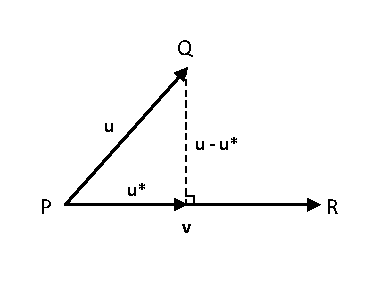
\includegraphics[width=4.1in]{1b.pdf}
				\end{figure}
				
			\item The triangle with vertices $P$, $Q$ and $R$ has the following dimensions,
				\begin{align}
					b&=\|\vec{PR}\|=\|\mathbf{v}\|=\sqrt{6} \notag \\
					h&=\|\mathbf{u}-\mathbf{u^*}\|=\sqrt{\frac{4}{9}+\frac{4}{9}+\frac{4}{9}}=
					\frac{2\sqrt{3}}{3} \notag
				\end{align}
				where $b$ is the base and $h$ is the (perpendicular) height. Its area is therefore
				\begin{align}
					A=\frac{1}{2}\hspace{0.1cm}bh=\frac{1}{2} \left(\sqrt{6}\right) \left(\frac{2\sqrt{3}}{3}						\right)=\sqrt{2} \notag
				\end{align}
				\begin{figure}[h]
					\centering
					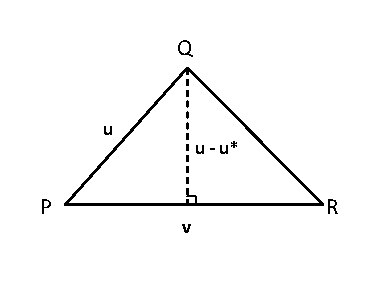
\includegraphics[width=4.1in]{1c.pdf}
				\end{figure}
				
			\item Let $\mathbf{w}=\vec{PS}=[2-(-1), 1-0, 2-0]=[3,1,2] = 3\mathbf{i}+\mathbf{j}+2\mathbf{k}$. 				The volume of the parallelepiped with sides given by the vectors $\vec{PQ}$, $\vec{PR}$
				and $\vec{PS}$ is given by the absolute value of the scalar triple product below.
					\begin{align}
						V= |\mathbf{u} \cdot (\mathbf{v} \times \mathbf{w})| \hspace{0.3cm} \text{where}
						\hspace{0.3cm} \mathbf{u} \cdot (\mathbf{v} \times \mathbf{w})= 
						\begin{vmatrix}
							\text{ } 2	&0	&0 \text{ } \\
							\text{ } 2	&1	&1 \text{ } \\
							\text{ } 3	&1	&2 \text{ }
						\end{vmatrix} \notag
					\end{align}
				Expanding by the first row, where $c_{ij}$ are the cofactors of $\mathbf{u} \cdot 
				(\mathbf{v} \times \mathbf{w}):$
					\begin{align}
						c_{11}=(-1)^{1+1}
						\begin{vmatrix}
							\text{ } 1	&1 \text{ } \\	
							\text{ } 1	&2 \text{ }
						\end{vmatrix} = 1(1\times2-1\times1)=1 \notag
					\end{align}	
				Hence $\mathbf{u} \cdot (\mathbf{v} \times \mathbf{w})=c_{11}\times2+c_{12}\times0+
				c_{13}\times0=1\times2=2 \hspace{0.3cm} \text{and} \hspace{0.3cm} V=|2|=2$ \\
				\begin{figure}[h]
					\centering
					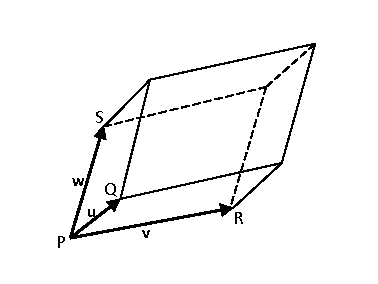
\includegraphics[width=4.1in]{1d.pdf}
				\end{figure}
				
		\end{enumerate}
		
	\item If $\mathbf{u}=u_1\mathbf{i}+u_2\mathbf{j}+u_3\mathbf{k}, \hspace{0.3cm}\mathbf{v}=v_1\mathbf{i}		+v_2 \mathbf{j}+v_3 \mathbf{k} \hspace{0.3cm} \text{and}\hspace{0.3cm}\mathbf{w}=w_1\mathbf{i}			+w_2 \mathbf{j}+w_3 \mathbf{k}$ \hspace{0.01cm} are three vectors in $\mathbb{R}^3$ then,
		\begin{align}
			\hspace{1cm}\mathbf{v} \times \mathbf{w}= 
			\begin{vmatrix}
				\text{ } \mathbf{i}&\mathbf{j}&\mathbf{k} \text{ } \\
				\text{ } v_1	&v_2	&v_3 \text{ } \\
				\text{ } w_1&w_2&w_3 \text{ }
			\end{vmatrix}
			=(v_2w_3-v_3w_2)\mathbf{i}-(v_1w_3-v_3w_1)\mathbf{j}+(v_1w_2-v_2w_1)\mathbf{k} \notag
		\end{align}
		Furthermore the vector triple product is given by
		\begin{align}
			\mathbf{u} \times(\mathbf{v} \times \mathbf{w})=
			\begin{vmatrix}
				\text{ } \mathbf{i}&\mathbf{j}&\mathbf{k} \text{ } \\
				\text{ } u_1&u_2&u_3 \text{ } \\
				\text{ } v_2w_3-v_3w_2 &-(v_1w_3-v_3w_1)&v_1w_2-v_2w_1 \text{ }
			\end{vmatrix} \notag
		\end{align} \\
		Thus the $\mathbf{i}$-component of $\mathbf{u} \times(\mathbf{v} \times \mathbf{w})$ is given 			by
		\begin{align}
			&=u_2(v_1w_2-v_2w_1)-u_3(v_3w_1-v_1w_3) \notag \\
			&=u_2v_1w_2-u_2v_2w_1-u_3v_3w_1+u_3v_1w_3 \notag \\
			&=v_1(u_2w_2+u_3w_3)-w_1(u_2v_2+u_3v_3) \notag \\
			&=v_1(\mathbf{u}\cdot\mathbf{w})-w_1(\mathbf{u}\cdot\mathbf{v}) \notag \\
			&=(\mathbf{u}\cdot\mathbf{w})v_1-(\mathbf{u}\cdot\mathbf{v})w_1 \notag
		\end{align}
		By symmetry, $(\mathbf{u}\cdot\mathbf{w})v_2-(\mathbf{u}\cdot\mathbf{v})w_2$ and $(\mathbf{u}			\cdot\mathbf{w})v_3-(\mathbf{u}\cdot\mathbf{v})w_3$ are the $\mathbf{j}$- and $\mathbf{k}$-
		components of $\mathbf{u} \times(\mathbf{v} \times \mathbf{w})$. Combining all three components
		therefore gives
		\begin{align}
			&=(\mathbf{u}\cdot\mathbf{w})(v_1+v_2+v_3)-(\mathbf{u}\cdot\mathbf{v})(w_1+w_2+w_3)
			\notag \\
			&=(\mathbf{u}\cdot\mathbf{w})\text{ }\mathbf{v}-(\mathbf{u}\cdot\mathbf{v})\text{ } \mathbf{w}
			\notag
		\end{align} \\
						
	\item I was unable to answer this successfully so my first attempt is shown instead, which assumes a 			slight variation to the phrasing of the question. \\
		\\
		Let $\angle P\hat{A}B = \theta$. Then,
		
		\begin{align}
			\|\vec{PA}\times\vec{AB}\|=\|\vec{PA}\|\|\vec{AB}\| \sin\theta \notag
		\end{align}
		
			\begin{figure}[h]
				\centering
				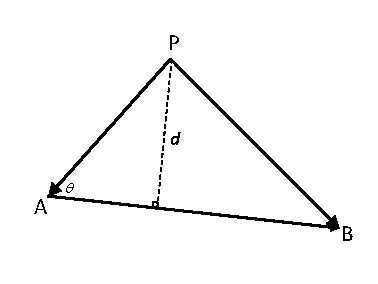
\includegraphics[width=4.1in]{3.pdf}
			\end{figure}
			
		If $d$ is the perpendicular distance from the point $P$ to the line $AB$, then the right-angle 
		$\triangle AQP$ (where $Q$ is a point on $\vec{AB}$ and $\angle A\hat{Q}P=90^\circ)$ implies \\
		\begin{align}
			\sin\theta=\frac{d}{\|\vec{PA}\|} \notag
		\end{align} \\
		
		It follows that $d=\|\vec{PA}\|\sin\theta$ and thus $\|\vec{PA}\times\vec{AB}\|=d\text{ }\|\vec{AB}\|$. 
		Rearranging gives \\
		\begin{align}
			d = \frac{\|\vec{PA}\times\vec{AB}\|}{\|\vec{AB}\|} \notag
		\end{align} \\
		
		However, if we were to answer the original question we produce the following diagram and 				calculations. \\
		\\
		\\
		\\
		\begin{figure}[h]
				\centering
				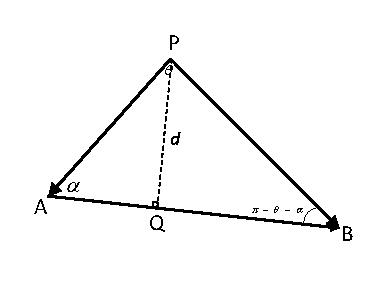
\includegraphics[width=4.1in]{3a.pdf}
			\end{figure}
		Let $\angle A\hat{P}B = \theta$. Then,
		\begin{align}
			\|\vec{PA}\times\vec{PB}\|=\|\vec{PA}\| \|\vec{PB}\| \sin\theta \hspace{0.1cm} \Rightarrow
			\hspace{0.1cm} \|\vec{PA}\|=\frac{\|\vec{PA}\times\vec{PB}\|}{ \|\vec{PB}\| \sin\theta} \notag
		\end{align} 
		If $\angle P\hat{A}B = \alpha$, it follows that 
			\begin{align}
			\sin\alpha=\frac{d}{\|\vec{PA}\|} \hspace{0.1cm} \Rightarrow \hspace{0.1cm} d&=\|\vec{PA}\|
			\sin\alpha \notag \\
			&=\frac{\|\vec{PA} \times \vec{PB}\| \sin\alpha}{\|\vec{PB}\| \sin\theta} \notag
		\end{align} 
		In order to show that	
		\begin{align}
			d &= \frac{\|\vec{PA}\times\vec{PB}\|}{\|\vec{AB}\|} \notag
		\end{align} 
		we must therefore show that 
		\begin{align}
			\frac{1}{\|\vec{AB}\|}=\frac{\sin\alpha}{\|\vec{PB}\| \sin\theta} \notag
		\end{align} \\
		which we fail to do due to some flaw in our reasoning.\\
		\\
		\\
		\\
	\item We solve the following systems of linear equations using Gauss-Jordan elimination. \\
	
		\begin{enumerate}
		
			\item
			\begin{align}
				\begin{array}{ccc|c}
					\text{ }\hspace{2.8cm}1&\text{ } \text{ }2&-4& \text{ } \text{ } \text{ }4 \\
					\text{ }\hspace{2.3cm}-3&-6& \text{ }12&-12
				\end{array} \notag
			\end{align} 
			
			\begin{align}
				\begin{array}{ccc|c}
					\text{ }\hspace{1.9cm}1&2&-4&4 \\ 
					-\frac{1}{3}R_2 \hspace{1cm} 1&2&-4&4
				\end{array} \notag
			\end{align} \\
			Hence the second equation is simply a multiple of the first.  It follows that the two planes 					coincide and that all points $(x,y,z)$ on the plane satisfy the pair of equations. \\
			
			\item 
			\begin{align}
				\begin{array}{ccc|c}
					\hspace{2.4cm} \text{ } \text{ } 1&-2& \text{ } \text{ } 1&-18 \\
					\hspace{2.4cm} \text{ } \text{ } 0& \text{ } \text{ } 2&-1& \text{ } \text{ } \text{ }8 \\
					\hspace{2.4cm} -4& \text{ } \text{ }5& \text{ } \text{ }9&-9
				\end{array} \notag
			\end{align} 
			\smallskip
			\begin{align}
				\begin{array}{ccc|c}
					 \hspace{2.7cm} 1&-2& \text{ } \text{ }1&-18 \\
					 \hspace{2.7cm} 0& \text{ } \text{ } 2&-1& \text{ } \text{ } \text{ }8 \\
					R_3+4R_1 \hspace{1.04cm}	0&-3& \text{ }13&-81
				\end{array} \notag
			\end{align} 
			\smallskip
			\begin{align}
				\begin{array}{ccc|c}
					R_1+R_2 \hspace{1cm} 1&\text{ } \text{ }0&\text{ } \text{ }0&-10 \\
					\hspace{2.5cm} 0& \text{ } \text{ } 2&-1& \text{ } \text{ } \text{ }8 \\
					\hspace{2.49cm} 0&-3& \text{ }13&-81
				\end{array} \notag
			\end{align} 
			\smallskip
			\begin{align}
				\begin{array}{ccc|c}
					\hspace{1.7cm} 1&\text{ } \text{ }0&\text{ } \text{ }0&-10 \\
					\frac{1}{2}R_2 \hspace{1cm} 0& \text{ } \text{ } 1&-\frac{1}{2}& \text{ } \text{ } \text{ }4 \\
					\hspace{1.72cm}0&-3& \text{ }13&-81
				\end{array} \notag
			\end{align} 
			\smallskip
			\begin{align}
				\begin{array}{ccc|c}
					\hspace{2.65cm}1&0&\text{ } \text{ }0&-10 \\
					\hspace{2.65cm} 0&1&-\frac{1}{2}& \text{ } \text{ } \text{ }4 \\
					R_3+3R_2 \hspace{1cm}0&0&\text{ }\frac{23}{2}&-69
				\end{array} \notag
			\end{align} 
			\smallskip
			\begin{align}
				\begin{array}{ccc|c}
					\hspace{2.2cm}1&0&\text{ } \text{ }0&-10 \\
					\hspace{2.2cm} 0&1&-\frac{1}{2}& \text{ } \text{ } \text{ }4 \\
					-\frac{1}{23}R_3 \hspace{1cm}0&0&-\frac{1}{2}&\text{ } \text{ } \text{ }3
				\end{array} \notag
			\end{align} 
			\smallskip
			\begin{align}
				\begin{array}{ccc|c}
					\hspace{2.5cm}1&0&\text{ } \text{ }0&-10 \\
					R_2-R_3\hspace{1cm} 0&1&\text{ } \text{ }0& \text{ } \text{ } \text{ }1 \\
					\hspace{2.5cm}0&0&-\frac{1}{2}&\text{ } \text{ } \text{ }3
				\end{array} \notag
			\end{align} 
			\smallskip
			\begin{align}
				\begin{array}{ccc|c}
					\hspace{2cm}1&0&0&-10 \\
					\hspace{2cm} 0&1&0& \text{ } \text{ } \text{ }1 \\
					-2R_3\hspace{1cm}0&0&1&-6
				\end{array} \notag
			\end{align} 
			\\
			Thus, $$x=-10, \hspace{0.3cm} y=1, \hspace{0.3cm} z=-6$$
			
			\item
			\begin{align}
				\begin{array}{ccc|c}
					\hspace{2.3cm} \text{ } \text{ } 0&\text{ } \text{ } 1&-4&8 \\
					\hspace{2.3cm} \text{ } \text{ } 2&-3&\text{ } \text{ }2&1 \\
					\hspace{2.3cm} \text{ } \text{ } 5&-8&\text{ } \text{ }7&1
				\end{array} \notag
			\end{align} 
			\smallskip
			\begin{align}
				\begin{array}{ccc|c}
					R_1+\frac{1}{2}R_2 \hspace{1cm} 1&-\frac{1}{2}&-3&\frac{17}{2} \\
					\hspace{2.5cm} \text{ } \text{ } 2&-3&\text{ } \text{ }2&1 \\
					\hspace{2.5cm} \text{ } \text{ } 5&-8&\text{ } \text{ }7&1
				\end{array} \notag
			\end{align} 
			\smallskip
			\begin{align}
				\begin{array}{ccc|c}
					\hspace{2.7cm} 1&-\frac{1}{2}&-3&\text{ } \text{ } \text{ } \frac{17}{2} \\
					R_2-2R_1\hspace{1cm}0&-2&\text{ } \text{ }8&-16 \\
					\hspace{2.4cm} \text{ } \text{ } 5&-8&\text{ } \text{ }7& \text{ } \text{ } \text{ } 1
				\end{array} \notag
			\end{align} 
			\smallskip
			\begin{align}
				\begin{array}{ccc|c}
					\hspace{2.7cm} 1&-\frac{1}{2}&-3&\text{ } \text{ } \text{ } \frac{17}{2} \\
					\hspace{2.7cm}0&-2&\text{ } \text{ }8&-16 \\
					R_3-5R_1\hspace{1cm} 0&-\frac{11}{2}&\text{ }22&-\frac{83}{2}
				\end{array} \notag
			\end{align} 
			\smallskip
			\begin{align}
				\begin{array}{ccc|c}
					R_1-\frac{1}{4}R_2\hspace{1cm}1&\text{ }\text{ }0&-5&\text{ }\text{ }\text{ }\frac{25}{2} 					\\
					\hspace{2.7cm}0&-2&\text{ } \text{ }8&-16 \\
					\hspace{2.7cm} 0&-\frac{11}{2}&\text{ }22&-\frac{83}{2}
				\end{array} \notag
			\end{align} 
			\smallskip
			\begin{align}
				\begin{array}{ccc|c}
					\hspace{2.05cm}1&\text{ }\text{ }0&-5&\text{ }\text{ }\text{ }\frac{25}{2} \\
					-\frac{1}{2}R_2 \hspace{1cm}0&\text{ } \text{ }1&-4&\text{ } \text{ } \text{ } 8 \\
					\hspace{2.05cm} 0&-\frac{11}{2}&\text{ }22&-\frac{83}{2}
				\end{array} \notag
			\end{align} 
			\smallskip
			\begin{align}
				\begin{array}{ccc|c}
					\hspace{2.15cm}1&0&-5&\frac{25}{2} \\
					\hspace{2.15cm}0&1&-4&8 \\
					-\frac{2}{11}R_3 \hspace{1cm} 0&1&-4&\frac{83}{11}
				\end{array} \notag
			\end{align} 
			\begin{align}
				\begin{array}{ccc|c}
					\hspace{2.45cm}1&0&-5&\text{ }\text{ }\frac{25}{2} \\
					\hspace{2.45cm}0&1&-4&\text{ } \text{ } 8 \\
					R_3-R_2 \hspace{1cm} 0&0&\text{ } \text{ } 0&-\frac{5}{11}
				\end{array} \notag
			\end{align} 
			\\
		The system is therefore inconsistent and there is no unique solution. \\
	
		\end{enumerate}
		
	\item A condition on the coefficients of $a_{ij}$ that guarantees a consistent system is
		\begin{align}
			a_{ij}=
			\begin{cases}
				1 \hspace{0.3cm} \text{if} \hspace{0.3cm} i=j \notag \\
				0  \hspace{0.3cm} \text{if} \hspace{0.3cm} i\ne j \notag
			\end{cases}
		\end{align}
		This reduces the general system of linear equations in three unknowns to the following 
		augmented matrix.
			\begin{align}
				\begin{array}{ccc|c}
					1&0&0&b_1 \\
					0&1&0&b_2 \\
					0&0&1&b_3
				\end{array} \notag
			\end{align} 
		Thus we have a unique solution in 
		$$x_1=b_1, \hspace{0.3cm} x_2=b_2, \hspace{0.3cm} x_3=b_3$$
		which implies that the system is consistent.
				
\end{enumerate}
	
\end{document}